\documentclass[10pt, unicode]{beamer}
\usepackage{fontspec}
\usepackage{polyglossia}
\setdefaultlanguage{english}
\usepackage{graphics}
\usepackage{graphicx}
\usepackage{subcaption}
\usepackage{float}
\usepackage{caption}
\usepackage{newfloat}

\graphicspath{{images/}}

\DeclareMathOperator{\sech}{sech}
\setsansfont{Fira Sans}
\title{Генерация текстурного меша и упаковка полигональных текстур в атлас}
\author[Терехов Д.Е.]{Студент группы Б8403а Терехов Дмитрий Евгеньевич\\
Руководитель:\\
Старший преподаватель кафедры информатики, математического и компьютерного моделирования\\
Александр Сергеевич Кленин}
\date{10 июля 2019}
\usetheme[progressbar=frametitle, numbering=fraction]{metropolis}
\makeatletter
        \setlength{\metropolis@progressinheadfoot@linewidth}{2pt}
    \makeatother
\begin{document}
    \begin{frame}[fragile]
        \titlepage
        \thispagestyle{empty}
    \end{frame}
    \begin{frame}
        \frametitle{Студия "Game Forest"}
        \begin{figure}[H]
            \centering
            \begin{subfigure}[l]{0.50\linewidth}
                \centering
                
\includegraphics[scale=0.15]{GAMEFOREST.png}
            \end{subfigure}
            \begin{subfigure}{0.49\linewidth}
                \begin{subfigure}{\linewidth}
                    \centering
                    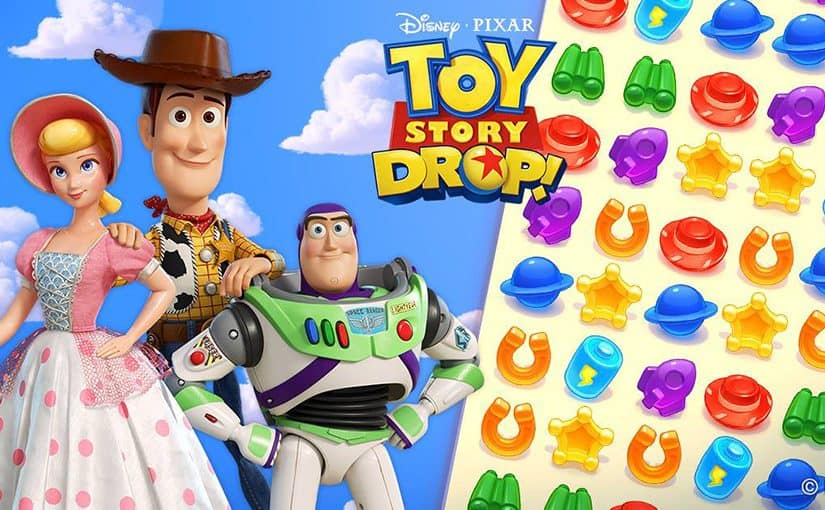
\includegraphics[scale=0.15]{TSD.jpg}
                \end{subfigure}
                \begin{subfigure}{\linewidth}
                    \centering
                    
\includegraphics[scale=0.260]{GD.jpg}
                \end{subfigure}
            \end{subfigure}
        \end{figure}
    \end{frame}
    \begin{frame}
        \frametitle{Игровой движок Citrus}
        \begin{figure}
            \centering
            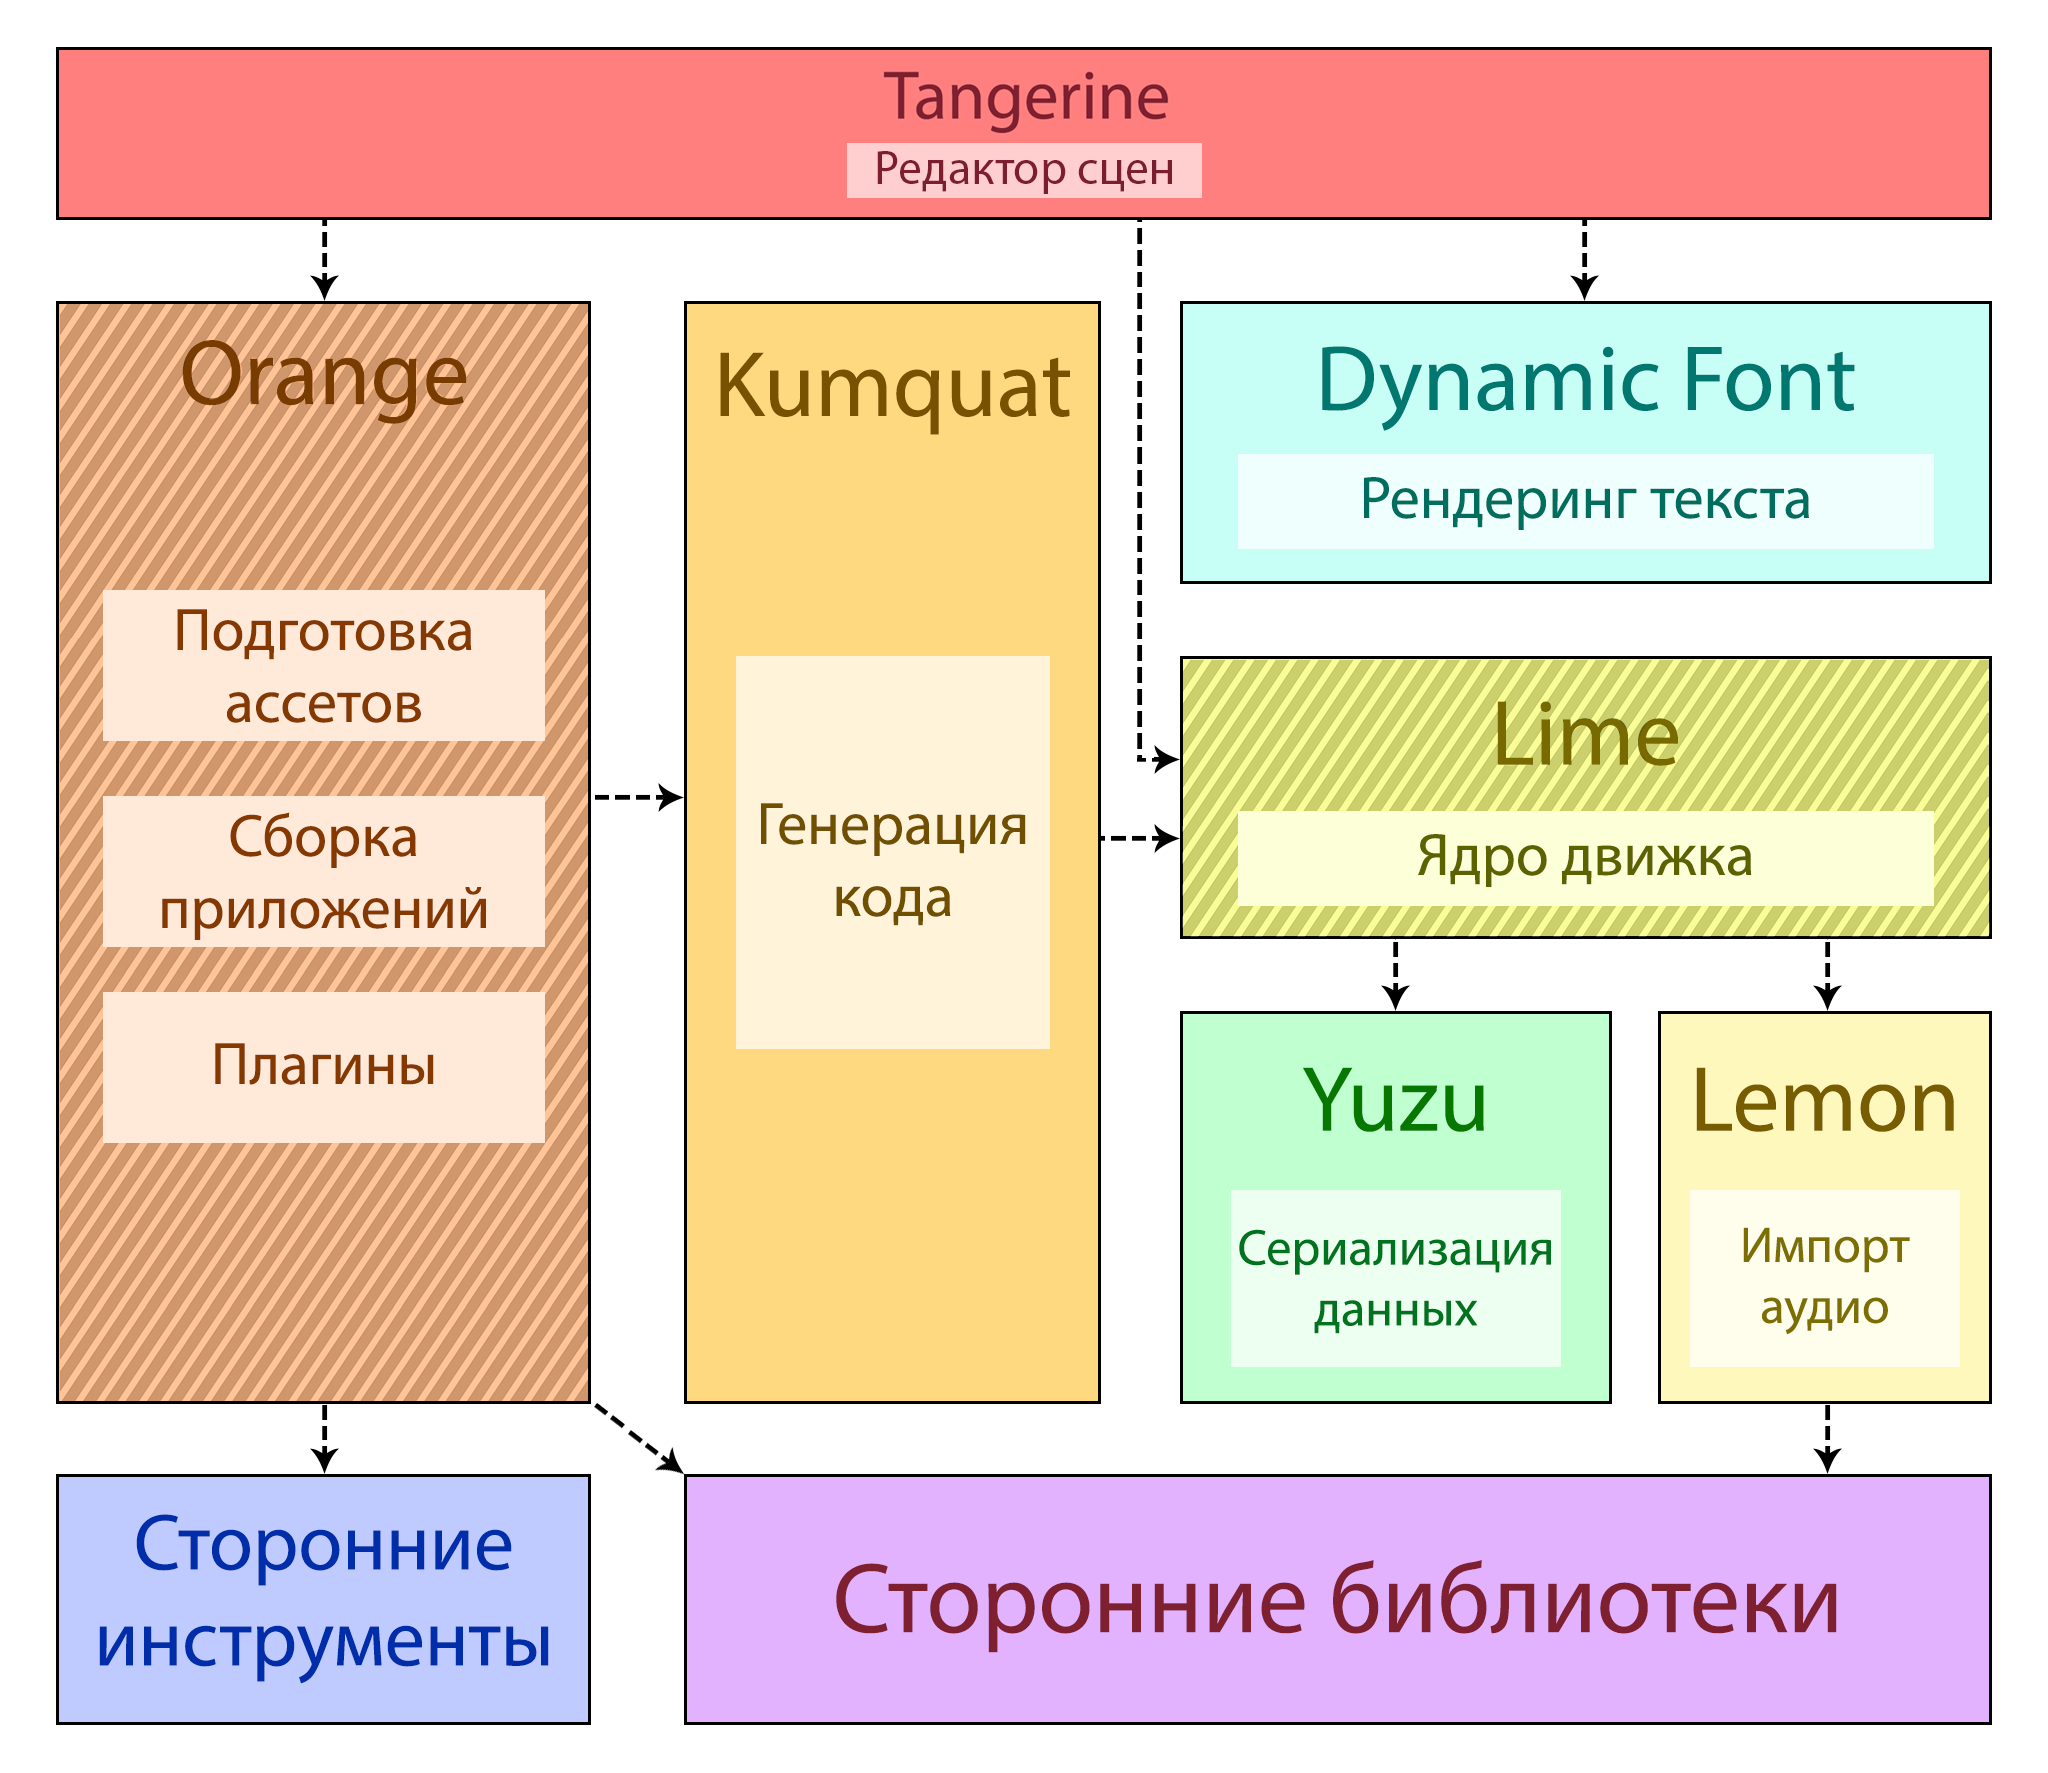
\includegraphics[width=\linewidth, height=.9\textheight, keepaspectratio]{CitrusArchitecture.png}
        \end{figure}
    \end{frame}
\end{document}
